% Lecture file created by newnote
% Class: Models of Theoretical Physics
% Professor: Azaele Sandro
% Date: 2025-10-17
\lecture{5}{Birth and death Markov processes}{2025-10-17}
\pagelayout{margin}
% --- Start writing here ---

\section{Birth and death Markov processes}
We discuss here a simple class of Markov processes, those that have a set of states that can be labeled with integers. We start from an even simpler discrete Markov process, the birth and death processes which occur in many applications. Then we will deduce results to more general cases.
We start from a situation that is very similar to the random walk. We assume discrete times $t=0, \Delta t, 2 \Delta t, \ldots$ discrete states $x=0, \pm 1, \pm 2 \ldots$ and that jumps are allowed only between nearest neighbors, i.e. from $n$ to $n \pm 1$. For $\Delta t \ll 1$ we call $b_{n} \geqslant 0$ the birth rate, i.e., $b_{n} \Delta t$ is the prob. to jump to $n+1$ at time $t+\Delta t$, given that at time $t$ the state was $n$. (notice that $b_{n}$ does not depend on time, though it could in principle. If it does not, we say that the process is homogeneous). Analogously, $d_{n} \geqslant 0$ is the death rate, i.e. $d_{n} \Delta t$ is the prob. to jump to $n-1$ at time $t+\Delta t$, given that at time $t$ the state was $n$.
We want to calculate the prob. $p(n, t+\Delta t)$ (the propagator).
\begin{figure}[H]
    \centering
    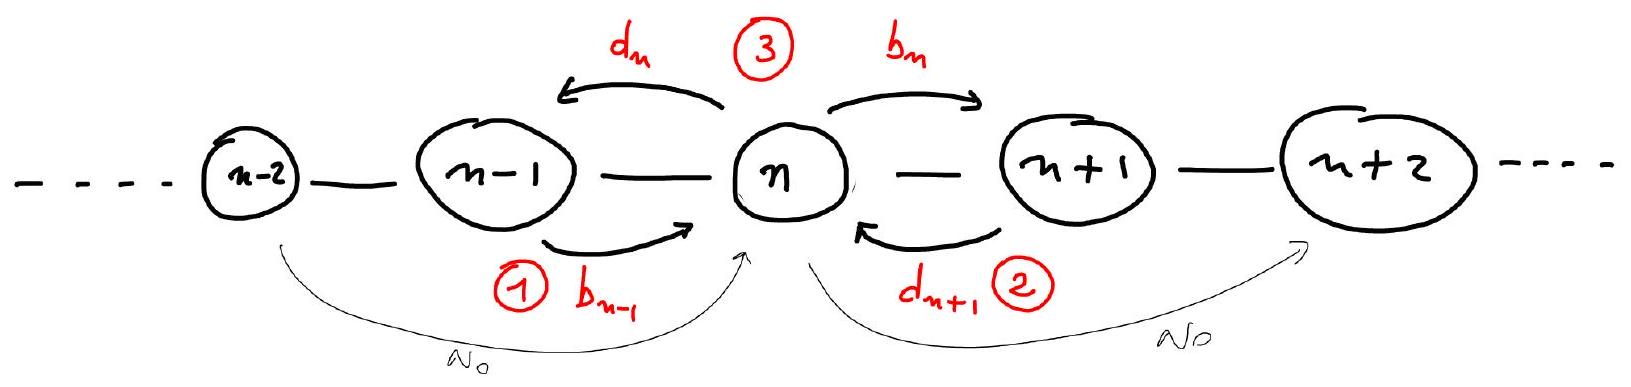
\includegraphics[width=\textwidth]{2025_10_17_3daf2a002a8f5936c90eg-01}
\end{figure}
\begin{DispWithArrows}[displaystyle, format=c]
    p(n, t+\Delta t)=b_{n-1} \Delta t p(n-1, t)+d_{n+1} \Delta t p(n+1, t)+\left[1-\left(b_{n}+d_{n}\right) \Delta t\right] p(n, t)
\end{DispWithArrows}
By Taylor expansions and then taking the limit $\Delta t \rightarrow 0$ we get
\begin{DispWithArrows}[displaystyle, format=c]
    \frac{\partial p_{n}}{\partial t}=b_{n-1} p_{n-1}(t)+d_{n+1} p_{n+1}(t)-\left(b_{n}+d_{n}\right) p_{n}(t)
\end{DispWithArrows}
This is called the master equation of the birth-death process or generation-recombination process.

A few observations:
\begin{enumerate}
    \item The M.E. is a gain-loss equation for the probabilities $p_{n}$;
    \item We have to equip eq. (1) with initial conditions. If We start with $P_{n, n_{0}}\left(t_{0}\right)=\delta_{n, n_{0}}$, then the M.E. is the equation of the propagator of the Markov process, that is
    \begin{DispWithArrows}[displaystyle, format=c]
        P_{n}(t) \equiv P\left(n, t \mid n_{0} t_{0}\right)
    \end{DispWithArrows}
    So one can show (exercise) that $p_{n}(t)$ satisfies the Chapman-Kolmogorov eq. in its differential form. More follows on this.
    \item We can introduce boundary conditions as well. For instance, if $N$ is a reflecting boundary,
    \begin{figure}[H]
        \centering
        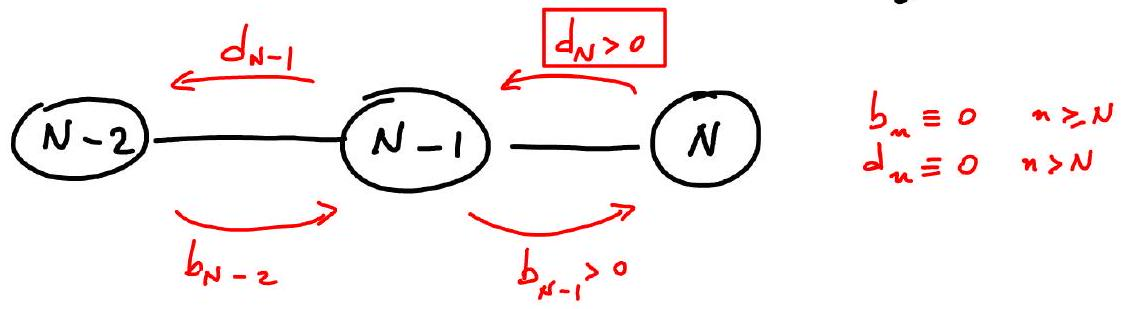
\includegraphics[width=\textwidth]{2025_10_17_3daf2a002a8f5936c90eg-02}
    \end{figure}
    then $b_{n} \equiv 0 \forall n \geqslant N, d_{n} \equiv 0 \forall n>N \quad\left(\right.$ for $n<N, b_{n}$ and $d_{n}$ are $\left.\geqslant 0\right)$ therefore if the state $N$ is reached, it can be left from one side only. $N$ is a reflecting state.

    If $N$ is an absorbing boundary,
    \begin{figure}[H]
        \centering
        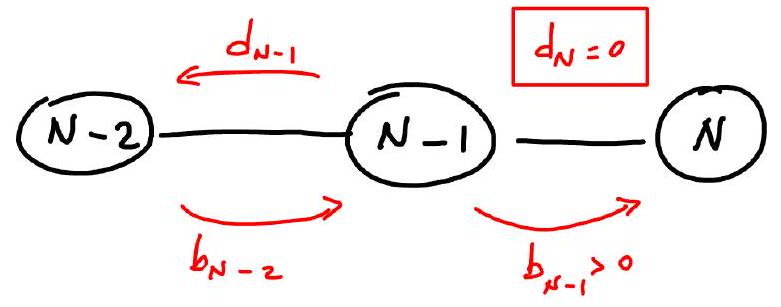
\includegraphics[width=\textwidth]{2025_10_17_3daf2a002a8f5936c90eg-03}
    \end{figure}
    here $d_{N}=0$ which is important, because when the state $N$ is reached, it can no longer be left. We say that $N$ is an absorbing state.
\end{enumerate}

\subsection*{Warning:}
Because of the b.c. We have to be careful with eq. (1) as it holds only when the boundary states are not hit, otherwise it must be changed.
\begin{enumerate}
    \setcounter{enumi}{3}
    \item Notice that eq. (1) is linear and deterministic; indeed we can define a matrix $\mathbb{W}$ whose entries are
    \begin{DispWithArrows}[displaystyle, format=c]
        \mathbb{W}_{m m^{\prime}}=d_{m^{\prime}} \delta_{m, m^{\prime}-1}+b_{m^{\prime}} \delta_{m, m^{\prime}+1}-\left(d_{m}+b_{m}\right) \delta_{m, n^{\prime}}
    \end{DispWithArrows}
    So, if we introduce the vector notation $[\vec{p}(t)]_{n} \equiv p_{n}(t)$ we can write eq. (1) as
    \begin{DispWithArrows}[displaystyle, format=c]
        \left\{\begin{array}{l}\dot{\vec{P}}(t)=\mathbb{W} \vec{P} \\ \vec{P}(0)=\vec{P}_{0}\end{array}\right.
    \end{DispWithArrows}
    and formally the solution reads $\vec{P}(t)=e^{\mathbb{W} t} \vec{P}_{0}$.
    The master equation defined in eq. (4b) holds in general for a continuous time, discrete Markov process as long as $\mathbb{W}$ satisfies the following properties:
    \begin{enumerate}
        \item $W_{n n^{\prime}} \geqslant 0$ for $n \neq n^{\prime}$
        \item $\sum_{m} \mathbb{W}_{m n^{\prime}}=0$ for each $n^{\prime}$ (no abs. bound.)
    \end{enumerate}
\end{enumerate}

\subsection*{The equations for the mean and the variance}
From eq. (1) one can simply derive the eqs. for the time evolution of the mean and the variance. We first multiply eq. (1) by $n$ and sum over $n$: $\langle n\rangle \equiv \sum_{-\infty}^{+\infty} n p_{n}(t)$
\begin{DispWithArrows}[displaystyle, format=c]
    \begin{aligned}
    \frac{d}{d t}\langle n\rangle & =\sum_{-\infty}^{+\infty}\left(n b_{n-1} p_{n-1}-n b_{n} p_{n}+n d_{n+1} p_{n+1}-n d_{n} p_{n}\right) \\
    & =\sum_{n}\left[(n+1) b_{n} p_{n}-n b_{n} p_{n}+(n-1) d_{n} p_{n}-n d_{n} p_{n}\right] \\
    & =\sum_{n}\left(b_{n}-d_{n}\right) p_{n}
    \end{aligned}
\end{DispWithArrows}
\begin{DispWithArrows}[displaystyle, format=c]
    \frac{d}{d t}\langle n\rangle=\left\langle b_{n}\right\rangle-\left\langle d_{n}\right\rangle \quad \begin{array}{ll}
     & \left\langle b_{n}\right\rangle \equiv \sum_{n} b_{n} p_{n} \\
     & \left\langle d_{n}\right\rangle \equiv \sum_{n} d_{n} p_{n}
    \end{array}
\end{DispWithArrows}
with some initial conditions. Notice that this equation has to be equipped with different equations if there is an absorbing or reflecting b.c. Can you find them?

For the evolution of the variance we have to derive an equation for the second moment $\left\langle n^{2}\right\rangle$. We first multiply eq. (1) by $n^{2}$ and then sum over $n$:
\begin{DispWithArrows}[displaystyle, format=c]
    \begin{aligned}
    \frac{d}{d t}\left\langle n^{2}\right\rangle & =\sum_{-\infty}^{+\infty} n^{2}\left(b_{n-1} p_{n-1}+\cdots\right)=\\
    & =\sum_{n}\left((n+1)^{2}-n^{2}\right) b_{n} p_{n}+\sum_{n}\left[(n-1)^{2}-n^{2}\right] d_{n} p_{n} \\
    & =\sum_{n}(2 n+1) b_{n} p_{n}+\sum_{n}(-2 n+1) d_{n} p_{n} \\
    & =2 \sum_{n} n\left(b_{n}-d_{n}\right) p_{n}+\sum_{n}\left(b_{n}+d_{n}\right) p_{n}
    \end{aligned}
\end{DispWithArrows}
Thus
\begin{DispWithArrows}[displaystyle, format=c]
    \frac{d}{d t}\left\langle n^{2}\right\rangle=2\left\langle n\left(b_{n}-d_{n}\right)\right\rangle+\left\langle b_{n}+d_{n}\right\rangle
\end{DispWithArrows}

\subsection*{The equilibrium distribution}
For birth and death process it is possible to calculate the equilibrium distribution of eq. (1) in general. This is not possible for more complicated discrete Markov processes.
We will calculate the distribution for a b/d process defined between 0 (ref. b.c.) and $\infty$.
We can define a stationary flux from $n-1$ to $n$:
\begin{figure}[H]
    \centering
    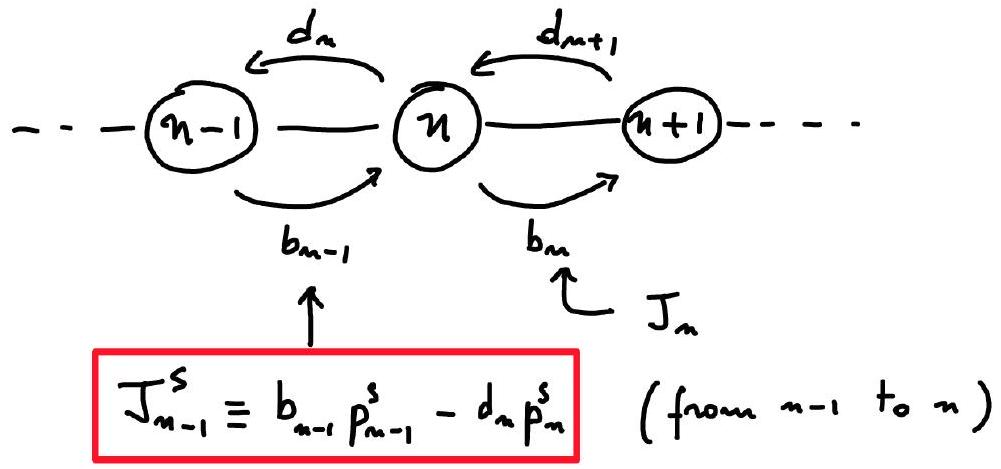
\includegraphics[width=0.5\textwidth]{2025_10_17_3daf2a002a8f5936c90eg-05}
\end{figure}
From eq. (1) we get then
\begin{DispWithArrows}[displaystyle, format=c]
    0=\underbrace{b_{n-1} p_{n-1}^{s}-d_{n} p_{n}^{s}}_{J_{n-1}}+\underbrace{d_{n+1} p_{n+1}^{s}-b_{n} p_{n}^{s}}_{-J_{n}}
\end{DispWithArrows}
hence $J_{n}=J_{n-1}=\ldots=J_{0} = b_{-1} p_{-1}^{s}-d_{0} p_{0}^{s}=0$ (ref. b.c. at $n=0$)
then
\begin{DispWithArrows}
    \begin{gathered}
    J_{n}=b_{n-1} p_{n-1}^{s}-d_{n} p_{n}^{s}=0 \Rightarrow b_{n-1} p_{n-1}^{s}=d_{n} p_{n}^{s} \quad \text{DETAILED BALANCE} \\
    p_{n}^{s}=\frac{b_{n-1}}{d_{n}} p_{n-1}^{s}=\frac{b_{n-1}}{d_{n}} \frac{b_{n-2}}{d_{n-1}} p_{n-2}^{s}=\ldots
    \end{gathered}
\end{DispWithArrows}
\begin{DispWithArrows}[displaystyle, format=c]
    p_{n}^{s}=\prod_{i=1}^{n} \frac{b_{i-1}}{d_{i}} p_{0}^{s} \quad \text { for } n=1,2, \ldots
\end{DispWithArrows}
because of normalization, $\left(p_{0}^{s}\right)^{-1}=1+\sum_{n=1}^{\infty} \prod_{i=1}^{n} \frac{b_{i-1}}{d_{i}}$; $p_{n}^{s}$ exists if $p_{0}^{s}<\infty$. The same approach can be used for a finite number of states $n=1, \ldots, N$.

\subsection*{Simple yet important birth and death processes}
\subsubsection*{Poisson process}
This process is defined by the rates $b_{n}=\lambda, d_{n}=0$, where $n=0,1, \ldots$ So the M.E. is
\begin{DispWithArrows}[displaystyle, format=c]
    \left\{\begin{array}{l}\dot{p}_{n}=\lambda\left(p_{n-1}-p_{n}\right) \\ p_{n}(0)=\delta_{n, 0}\end{array}\right.
\end{DispWithArrows}
Ex: show that the mean satisfies the eq. $\frac{d}{d t}\langle n\rangle=\lambda$ and so $\langle n(t)\rangle=n_{0}+\lambda t$ if $p_{n}(0)=\delta_{n, n_{0}}$.

We solve eq. (8) with the method of the generating function:
\begin{DispWithArrows}[displaystyle, format=c]
    g(z, t) \equiv \sum_{n=0}^{\infty} z^{n} p_{n}(t)
\end{DispWithArrows}
So from eq. (8) we get an eq. for $g$:
\begin{DispWithArrows}[displaystyle, format=c]
    \left\{\begin{array}{l}\frac{\partial}{\partial t} g(z, t)=\lambda(z-1) g(z, t) \quad\left(g(1, t)=\sum_{n} p_{n}(t)=1\right) \\ g(z, 0)=\sum_{n} z^{n} \delta_{n, 0}=1\end{array}\right.
\end{DispWithArrows}
The solution of (9) is then
\begin{DispWithArrows}[displaystyle, format=c]
    g(z, t)=e^{\lambda(z-1) t}=e^{-\lambda t} \sum_{n=0}^{\infty} \frac{(\lambda t)^{n}}{n!} z^{n}
\end{DispWithArrows}
hence
\begin{DispWithArrows}[displaystyle, format=c]
    p_{n}(t)=e^{-\lambda t} \frac{(\lambda t)^{n}}{n!}
\end{DispWithArrows}
Show that $\operatorname{var}(n(t))=\lambda t$.

\subsubsection*{Radioactive decay}
Initially the system consists of $N_{0}$ radioactive particles which decay at rate $\gamma$. Therefore, if at time $t$ there are $n$ surviving particles, then in the following $\Delta t$ time the probability of one decay is $\gamma n \Delta t$ and more than one decay is $o(\Delta t)$. Thus $d_{n}=\gamma n$ and $b_{n}=0$ and the M.E. is
\begin{DispWithArrows}[displaystyle, format=c]
    \left\{\begin{array}{l}\dot{p}_{n}=\gamma(n+1) p_{n+1}(t)-\gamma n p_{n}(t) \quad n=0,1 \ldots N_{0}-1 \quad \text{a.b.c. at } n=0 . \\ \dot{p}_{N_{0}}=-\gamma N_{0} p_{N_{0}}(t) \\ p_{n}(0)=\delta_{n, N_{0}}\end{array}\right.
\end{DispWithArrows}
Ex: show that $\frac{d}{d t}\langle n\rangle=-\gamma\langle n\rangle$, so $\langle n(t)\rangle=N_{0} e^{-\gamma t}$.
With the generating function $g(z, t)=\sum_{n=0}^{N_{0}} z^{n} p_{n}(t)$ we get
\begin{DispWithArrows}[displaystyle, format=c]
    \frac{\partial g(z, t)}{\partial t}=\gamma(1-z) \frac{\partial}{\partial z} g(z, t) \quad \begin{aligned} & g(1, t)=1 \\ & g(z, 0)=z^{N_{0}} \end{aligned}
\end{DispWithArrows}
Notice that $h(z, t)=\varepsilon(t)(1-z)+1$ leads to $\dot{\varepsilon}=-\gamma \varepsilon$, namely $\varepsilon(t)=\varepsilon_{0} e^{-\gamma t}$, so $h(1, t)=1$, but $h(z, 0)=\varepsilon_{0}(1-z)+1 \neq z^{N_{0}}$. However, take $g$ as a function of $h$, i.e. $g(z, t)=f(h(z, t))$, we get from (11)
\begin{DispWithArrows}[displaystyle, format=c]
    \frac{\partial g}{\partial t}=\frac{d f}{d h} \frac{\partial h}{\partial t} \quad , \quad \frac{\partial g}{\partial z}=\frac{d f}{d h} \frac{\partial h}{\partial z}
\end{DispWithArrows}
and $\frac{d f}{d h}$ simplifies, because it occurs on both sides of eq. (11). We can then use $f$ to satisfy the i.c.: $f(a)=a^{N_{0}}$ does the job. We take $g=\left(\varepsilon_{0} e^{-\gamma t}(1-z)+1\right)^{N_{0}}$ where $\varepsilon_{0}=-1$. Eventually, the sol, is
\begin{DispWithArrows}[displaystyle, format=c]
    g(z, t)=\left(e^{-\gamma t}(z-1)+1\right)^{N_{0}}
\end{DispWithArrows}
We have now to invert this relation to get $p_{n}(t)$
\begin{DispWithArrows}[displaystyle, format=c]
    g(z, t)=\left(e^{-\gamma t} z+\left(1-e^{-\gamma t}\right)\right)^{N_{0}}=\sum_{n=0}^{N_{0}}\binom{N_{0}}{n}\left(1-e^{-\gamma t}\right)^{N_{0}-n} e^{-n \gamma t} z^{n}
\end{DispWithArrows}
which gives
\begin{DispWithArrows}[displaystyle, format=c]
    p_{n}(t)=\binom{N_{0}}{n} e^{-n \gamma t}\left(1-e^{-\gamma t}\right)^{N_{0}-n}
\end{DispWithArrows}
We can interpret this eq. in this way: $e^{-n \gamma t}$ is the prob. that $n$ particles have survived (i.e., not decayed yet) by time $t,\left(1-e^{-\gamma t}\right)^{N_{0}-n}$ is the prob. that $N_{0}-n$ particles have decayed by time $t$. We also need the factor $\binom{N_{0}}{n}$ because the specific identity of the particles is not important, then there are $\binom{N_{0}}{n}$ ways to select $n$ surviving particles out of $N_{0}$.

\subsubsection*{Furry process}
A cosmic electron enters an absorbing material (like lead...) and branches into multiple particles (an electron may emit a photon which may then produce an $e^{+}-e^{-}$ pair). So a cascade of secondary particles is produced which generates a shower of final particles. This process can be described by a birth and death process where $b_{n}=\gamma n$ and $d_{n}=0, n=1,2, \ldots$
The M.E. is then
\begin{DispWithArrows}[displaystyle, format=c]
    \left\{\begin{array}{l}\dot{p}_{n}=\gamma(n-1) p_{n-1}-\gamma n p_{n} \\ p_{n}(0)=\delta_{n, 1}\end{array}\right.
\end{DispWithArrows}
Show as before that
\begin{DispWithArrows}[displaystyle, format=c]
    \begin{aligned}
    & \langle n(t)\rangle=e^{\gamma t} \\
    & \operatorname{Var}(n(t))=e^{\gamma t}\left(e^{\gamma t}-1\right)
    \end{aligned}
\end{DispWithArrows}
Finally:
\begin{DispWithArrows}[displaystyle, format=c]
    p_{n}(t)=e^{-\gamma t}\left(1-e^{-\gamma t}\right)^{n-1}
\end{DispWithArrows}
try to interpret the result.

\subsubsection*{The contact process}
Let us assume that a population of $N$ individuals can be divided into two categories according to whether they are infected or not (but are susceptible any way). If an indiv. has not yet caught the infection, may catch it from any of of the $n$ infected ones (uniformly at random).
We can write down the transition rate from $n$ to $n+1$ infected individuals; if the number of infected ind. increases by one, then one healthy ind. must get in contact with an infected one:
\begin{enumerate}
    \item first, we have to pick one healthy indiv.
    \begin{DispWithArrows}
        b_{n}=\tilde{\beta} \frac{N-n}{N} \frac{n}{N-1}=\frac{\beta}{N} n(N-n)
    \end{DispWithArrows}
    \item second, the healthy ind. have to encounter an infected one.
\end{enumerate}
We then assume that an infected individual recovers at rate $\gamma$. then the transition rate from state $n$ to $n-1$ is $d_{n}=\gamma n$. Notice that $b_{0}=0=d_{0}$ ($n=0$ is an absorbing state) and $b_{N}=0, d_{N} \neq 0$ ($n=N$ is a reflecting state) and we have to set $d_{N+1}=0$.
Notice that the rates $b_{n}$ and $d_{n}$ can be written as a function of $x=\frac{n}{N}: b_{x}=N \beta x(1-x), d_{x}=N \gamma x$.
As $N$ becomes large, the variations in $n$ become small and so one hopes to describe $x$ as a continuous variable. Making this limit rigorous is tricky (Kurtz's theorem), but one can anyway guess the limiting equation. the important assumption is the existence of a typical scale of the system (in this case $N$) and that the parameters (here $\beta$ and $\gamma$) scale appropriately with $N$.

The master equation has a form
\begin{DispWithArrows}[displaystyle, format=c]
    \dot{q}_{n}(t)=b_{\frac{n-1}{N}} q_{n-1}+d_{\frac{n+1}{N}} q_{n+1}-\left(b_{\frac{n}{N}}+d_{\frac{n}{N}}\right) q_{n}
\end{DispWithArrows}
In the continuous limit $q_{n}(t)$ becomes a PDF of $x$, so we write
\begin{DispWithArrows}[displaystyle, format=c]
    q_{n}(t)=\frac{1}{N} p(x, t) \quad \text { for large } N
\end{DispWithArrows}
So eq. (15) becomes
\begin{DispWithArrows}[displaystyle, format=c]
    \dot{p}(x, t)=b_{x-\frac{1}{N}} p\left(x-\frac{1}{N}, t\right)+d_{x+\frac{1}{N}} p\left(x+\frac{1}{N}, t\right)-\left(b_{x}+d_{x}\right) p(x, t)
\end{DispWithArrows}
As $\frac{1}{N}$ is small, we can Taylor expand eq. (16):
\begin{DispWithArrows}[displaystyle, format=c]
    \begin{aligned}
    & b_{x-\frac{1}{N}} p\left(x-\frac{1}{N}\right)-b_{x} p(x)=-\frac{1}{N} \frac{d}{d x}\left(b_{x} p_{x}\right)+\frac{1}{2} \frac{1}{N^{2}} \frac{d^{2}}{d x^{2}}\left(b_{x} p_{x}\right)+\text { h.o.t. } \\
    & d_{x+\frac{1}{N}} p\left(x+\frac{1}{N}\right)-d_{x} p(x)=\frac{1}{N} \frac{d}{d x}\left(d_{x} p_{x}\right)+\frac{1}{2} \frac{1}{N^{2}} \frac{d^{2}}{d x^{2}}\left(d_{x} p_{x}\right)+\text { h.o.t. }
    \end{aligned}
\end{DispWithArrows}
Therefore
\begin{DispWithArrows}[displaystyle, format=c]
    \dot{p}(x, t)=-\frac{1}{N} \frac{\partial}{\partial x}\left[\left(b_{x}-d_{x}\right) p_{x}\right]+\frac{1}{2 N^{2}} \frac{\partial^{2}}{\partial x^{2}}\left[\left(b_{x}+d_{x}\right) p_{x}\right]+\text { h.o.t. }
\end{DispWithArrows}
as $b_{x}=N \beta x(1-x)$ and $d_{x}=N \gamma x$ we get the F.P. equation
\begin{DispWithArrows}[displaystyle, format=c]
    \dot{p}(x, t)=-\frac{\partial}{\partial x}[(\beta x(1-x)-\gamma x) p]+\frac{1}{2 N} \frac{\partial^{2}}{\partial x^{2}}[(\beta x(1-x)+\gamma x) p]
\end{DispWithArrows}
which corresponds to an Itô SDE: ($0<x<1$)
\begin{DispWithArrows}[displaystyle, format=c]
    d x=(\beta x(1-x)-\gamma x) d t+\sqrt{\frac{\beta x(1-x)+\gamma x}{N}} d B(t)
\end{DispWithArrows}
Fluctuations are of order $N^{-1 / 2}$.

In general, although the equation and its derivation are not rigorous, a birth and death process may be well approximated by the F.P. equation
\begin{DispWithArrows}[displaystyle, format=c]
    \dot{p}(x, t)=-\frac{\partial}{\partial x}\left[\left(b_{x}-d_{x}\right) p_{x}\right]+\frac{1}{2} \frac{\partial^{2}}{\partial x^{2}}\left[\left(b_{x}+d_{x}\right) p_{x}\right]
\end{DispWithArrows}
at least in some region of the parameter space. It is anyway expected that eq. (19) is very inaccurate close to (possible) boundaries or when $N$ (or other typical param.) is small. This approx is called Kramers-Moyal expansion and has several generalizations. Other more rigorous approximations exist (like the van Kampen approximation (see p. 244, van Kampen) or the WKB expansion... which are more accurate but more difficult as well.

Back to the contact process.
The mean of the infected individuals, $\rho(t) \equiv \mathbb{E}(x(t))$, satisfies (see eq. (18b))
\begin{DispWithArrows}[displaystyle, format=c]
    \dot{\rho}=(\beta-\gamma) \rho-\beta \mathbb{E}\left(x(t)^{2}\right)
\end{DispWithArrows}
This equation is not closed and cannot be solved, unless we know the behavior of $\mathbb{E}\left(x^{2}\right)$. The mean depends on the fluctuations. However, the eq. for $\mathbb{E}\left(x^{2}\right)$ depends on $\mathbb{E}\left(x^{3}\right)$, so we obtain an infinite chain of equations which cannot be solved unless we solve the full F.P. equation.
One way to obtain some information is to resort to the moment closure: if fluctuations are small, then
\begin{DispWithArrows}
    \mathbb{E}\left(x^{2}(t)\right) \simeq \mathbb{E}(x(t))^{2}=\rho(t)^{2}
\end{DispWithArrows}
Under this approximation
\begin{DispWithArrows}[displaystyle, format=c]
    \dot{\rho}=(\beta-\gamma) \rho-\beta \rho^{2}
\end{DispWithArrows}
which is a logistic equation that can be solved as we have seen at the beginning of the course.
There are two steady states ($\dot{\rho}=0$): $\rho^{*}=0$ and $\bar{\rho}=\frac{\beta-\gamma}{\beta}$. What is their meaning?
Let's look at their stability:
\begin{DispWithArrows}[displaystyle, format=c]
    \frac{d \dot{\rho}}{d \rho}=\beta-\gamma-\left.2 \beta \rho\right|_{\rho=\rho^{s t}}=\left\{\begin{array}{cc}
    \beta-\gamma & \rho=\rho^{*}=0 \\ \gamma-\beta & \rho=\bar{\rho}=\frac{\beta-\gamma}{\beta}\end{array}\right.
\end{DispWithArrows}
\begin{itemize}
    \item Therefore $\rho=0$ is stable as $\beta<\gamma$ (and $\bar{\rho}$ is unstable)
    \begin{figure}[H]
        \centering
        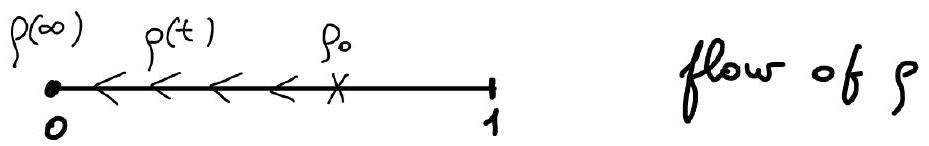
\includegraphics[width=0.5\textwidth]{2025_10_17_3daf2a002a8f5936c90eg-12}
    \end{figure}
    after some time, the eq. is well approximated by
    \begin{DispWithArrows}[displaystyle, format=c]
        \dot{\rho}=(\beta-\gamma) \rho \quad \rightarrow \rho(t)=\tilde{\rho} e^{-|\beta-\gamma| t} \rho \rightarrow_{t}
    \end{DispWithArrows}
    \item Viceversa, $\bar{\rho}=\frac{\beta-\gamma}{\beta}(>0)$ is stable as $\beta>\gamma$ (and $\rho=0$ is unstable)
    \begin{figure}[H]
        \centering
        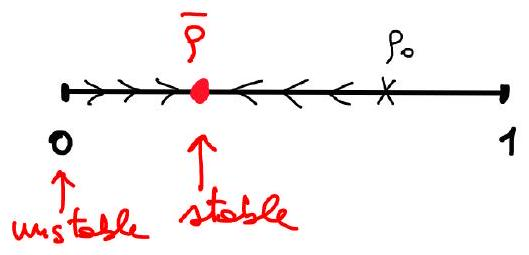
\includegraphics[width=0.5\textwidth]{2025_10_17_3daf2a002a8f5936c90eg-12(1)}
    \end{figure}
    after some time, the eq. is well approximated by $\rho(t)=\bar{\rho}+y(t)$ ($y \ll \bar{\rho}$)
    \begin{DispWithArrows}[displaystyle, format=c]
        \dot{\rho}=-(\beta-\gamma)(\bar{\rho}-\rho) \quad \rightarrow \quad \rho(t)=\bar{\rho}+\tilde{\rho} e^{-|\beta-\gamma| t}
    \end{DispWithArrows}
\end{itemize}
\begin{figure}[H]
    \centering
    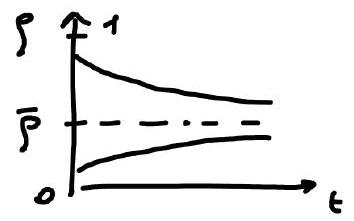
\includegraphics[width=0.5\textwidth]{2025_10_17_3daf2a002a8f5936c90eg-12(2)}
\end{figure}
So the characteristic time scale is $|\beta-\gamma|^{-1}$ in both cases.
Of course this is summarized by the full solution:
\begin{DispWithArrows}[displaystyle, format=c]
    \rho(t)=\frac{\bar{\rho}}{1+\left(\frac{\bar{\rho}}{\rho_{0}}-1\right) e^{(\gamma-\beta) t}}=\frac{(\beta-\gamma) \rho_{0}}{\beta \rho_{0}+\left(\beta-\gamma-\beta \rho_{0}\right) e^{(\gamma-\beta) t}}
\end{DispWithArrows}
where $\rho_{0}$ is the initial condition for the density ($0<\rho_{0}<1$) of infected individuals.
The phase diagram of this process reads:
\begin{figure}[H]
    \centering
    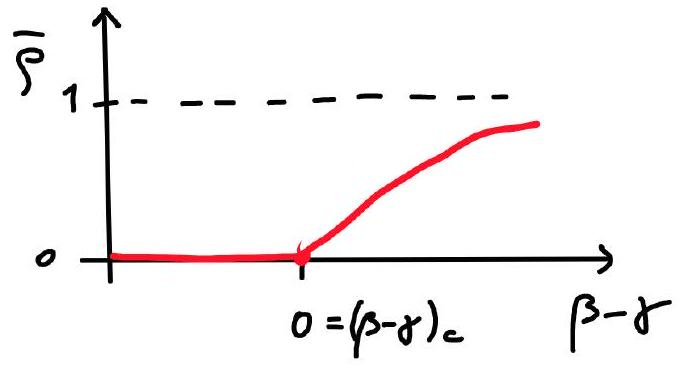
\includegraphics[width=0.5\textwidth]{2025_10_17_3daf2a002a8f5936c90eg-13}
\end{figure}
\begin{DispWithArrows}[displaystyle, format=c]
    \begin{gathered}
    \bar{\rho} \sim(\beta-\gamma)^{1} \\
    \beta>\gamma
    \end{gathered}
\end{DispWithArrows}
At the critical point $\beta=\gamma$:
\begin{DispWithArrows}[displaystyle, format=c]
    \dot{\rho}=-\beta \rho^{2} \quad \rightarrow \quad \rho(t)=\frac{\rho_{0}}{1+\beta t} \sim \frac{1}{t} \quad t \gg \beta^{-1}
\end{DispWithArrows}
the decay is no longer exponential but power law: critical slowing down.

Exercise: the discrete random walk in continuous time is governed by the master equation (symmetric R.W.)
\begin{DispWithArrows}[displaystyle, format=c]
    \dot{p}_{n}=p_{n+1}+p_{n-1}-2 p_{n} \quad p_{n}(0)=\delta_{n, 0}
\end{DispWithArrows}
Show that the generating function $F(z, t)=\sum_{-\infty}^{+\infty} z^{n} p_{n}(t)$ satisfies
\begin{DispWithArrows}[displaystyle, format=c]
    \dot{F}=\left(z+\frac{1}{z}-2\right) F
\end{DispWithArrows}
so the solution is $F(z, t)=\exp \left[t\left(z+z^{-1}-2\right)\right]$. From this find
\begin{DispWithArrows}[displaystyle, format=c]
    p_{n}(t)=e^{-t} \sum_{\substack{l \geqslant 0 \\ l+m \geqslant 0}} \frac{t^{2 l+m}}{(l+m)!l!}
\end{DispWithArrows}
Find the K.M. expansion of the M.E. and find its solution.

\subsection*{A simple chemical reaction}
Consider the reaction
\begin{DispWithArrows}[displaystyle, format=c]
    X \underset{k_{2}}{\stackrel{k_{1}}{\rightleftarrows}} A
\end{DispWithArrows}
where the product $A$ is not affected by $x$ and it does not decrease its quantity even though it produces particles at rate $k_{2}$. We are interested into the stochastic evolution of $X$: the r.v. $n$. From a simple application of the mass action law we get the evolution of the deterministic value $\rho(t)=\mathbb{E}(n(t))$:
\begin{DispWithArrows}[displaystyle, format=c]
    \dot{\rho}=-k_{1} \rho+k_{2} a
\end{DispWithArrows}
where $a$ is a constant.

We want now to get information about the fluctuations: If at time $t$ there are $n$ particles of type $x$, then the prob. that at time $t+\Delta t$ there is one more is given by $k_{2} a \Delta t$, and one less is $k_{1} n \Delta t$. So we get a birth and death process with rates
\begin{DispWithArrows}[displaystyle, format=c]
    \begin{aligned}
    & b_{n}=k_{2} a \equiv b \quad(\text { a constant }) \\
    & d_{n}=k_{1} n
    \end{aligned}
\end{DispWithArrows}
where $n=0,1, \ldots$
It is not difficult to find that the equilibrium distribution of $n$ (from eq. (7))
\begin{DispWithArrows}[displaystyle, format=c]
    p_{n}^{s t}=\frac{\lambda^{n}}{n!} e^{-\lambda} \quad \lambda=\frac{k_{2}a}{k_{1}}
\end{DispWithArrows}
what is the difference between this solution and eq. (10)?
The average is also (from eq. (5))
\begin{DispWithArrows}[displaystyle, format=c]
    \frac{d}{d t}\langle n\rangle=b-k_{1}\langle n\rangle
\end{DispWithArrows}
which is like eq. 23.
Ex: find the M.E. for the chemical reaction $A+x \xrightarrow{k_{1}} 2 x, x \stackrel{k_{2}}{\stackrel{k_{3}}{\rightleftarrows}} B$. and compare the results with those from the law of mass action.

\subsection*{Exact simulation of a birth and death process: the Gillespie's algorithm}
The M.E. in eq. (1) governs a b/d process whose trajectories can be generated exactly (up to machine numerical errors). The M.E. includes all the info we need as it defines the process itself. We know that it is a Markov process therefore the information that we possess at time $t$ is enough to define what happens in the future.
We need two pieces of info to generate a path:
\begin{enumerate}
    \item What is the time of the next event (either birth or death)?
    \item What is the nature of the event, given that it occurs? namely, what is the probability that it is a birth/death?
\end{enumerate}
If we can answer these two questions then we know when and how the path changes.
Let's define $q_{0}(\tau \mid n)$ as the probability that no events will occur within the interval $[0, \tau)$, given that the system was in the state $n$ at time $t=0$ (as the process is homogeneous, $t=0$ is not a restrictive assumption).
Notice that if $T$ is the (random) time when the next event (birth or death) will occur, then $q_{0}(\tau \mid n)=P(T>\tau \mid n)$.
We build up an equation for $q_{0}(\tau \mid n)$ by using the Markov assumption and that the process is a b/d process:
The prob. that there are no events in the interval $[0, \tau+\Delta \tau)$ is given by the prob. that no events occur within $[0, \tau)$ and neither occur in $[\tau, \tau+\Delta \tau)$:
\begin{DispWithArrows}[displaystyle, format=c]
    q_{0}(\tau+\Delta \tau \mid n)=q_{0}(\tau \mid n)\left(1-b_{n} \Delta \tau-d_{n} \Delta \tau\right)
\end{DispWithArrows}
Therefore as $\Delta \tau \rightarrow 0$
\begin{DispWithArrows}
    \left\{\begin{aligned}
    \frac{d q_{0}(\tau \mid n)}{d \tau} & =-\left(b_{n}+d_{n}\right) q_{0}(\tau \mid n) \\
    q_{0}(0 \mid n) & =1
    \end{aligned}\right.
\end{DispWithArrows}
hence
\begin{DispWithArrows}[displaystyle, format=c]
    q_{0}(\tau \mid n)=e^{-\left(b_{n}+d_{n}\right) \tau}
\end{DispWithArrows}
Now we can calculate $q_{+}(\tau \mid n) \Delta \tau$, namely, the probability that a birth occurs between $\tau$ and $\tau+\Delta \tau$ if the system was in state $n$. This is simply
\begin{DispWithArrows}[displaystyle, format=c]
    q_{+}(\tau \mid n) \Delta \tau=e^{-\left(b_{n}+d_{n}\right) \tau} b_{n} \Delta \tau
\end{DispWithArrows}
prob. of no events up to time $\tau$ prob. of 1 birth event between $\tau$ and $\tau+\Delta \tau$

Therefore the PDF is
\begin{DispWithArrows}[displaystyle, format=c]
    q_{+}(\tau \mid n)=b_{n} e^{-\left(b_{n}+d_{n}\right) \tau}
\end{DispWithArrows}
and for a death event
\begin{DispWithArrows}[displaystyle, format=c]
    q_{-}(\tau \mid n)=d_{n} e^{-\left(b_{n}+d_{n}\right) \tau}
\end{DispWithArrows}
and the PDF of any event (either birth or death) is therefore
\begin{DispWithArrows}[displaystyle, format=c]
    q_{1}(\tau \mid n)=\left(b_{n}+d_{n}\right) e^{-\left(b_{n}+d_{n}\right) \tau}
\end{DispWithArrows}
This means that the PDF of an event is exponentially distributed with mean time $\langle\tau(n)\rangle=\left(b_{n}+d_{n}\right)^{-1}$ (show this). Of course, we assume that the state $n$ is not absorbing, i.e. $b_{n}+d_{n}>0$.

Now $q_{+}(\tau \mid n) \Delta \tau=\left(\begin{array}{c} \text{prob. of a birth event,} \\ \text{given that an event occurs} \\ \text{between } \tau \text{ and } \tau+\Delta \tau\end{array}\right)\binom{\text { prob. that an event occurs }}{\text { between } \tau \text{ and } \tau+\Delta \tau}$
From eqs. (27) we get
\begin{DispWithArrows}[displaystyle, format=c]
    q_{+}(\tau \mid n) \Delta \tau=\frac{b_{n}}{b_{n}+d_{n}}\left(b_{n}+d_{n}\right) e^{-\left(b_{n}+d_{n}\right) \tau} \Delta \tau
\end{DispWithArrows}
prob. of a birth event, given that an event occurs between $\tau$ and $\tau+\Delta \tau$ when the state is $n$
prob. that an event occurs (birth or death) between $\tau$ and $\tau+\Delta \tau$ when the state is $n$

Eq. (30) suggests an algorithm for simulating a path from the master equation (1):

\subsection*{Gillespie's algorithm}
(1) Initialize the system at time $t=0$, starting at state $n_{0}$:
(2) If $b_{n}+d_{n}>0$, generate the time $\tau$ when the next event will occur. So you have to draw a random number from the exponential distribution (29), or equivalently (show this)
\begin{DispWithArrows}[displaystyle, format=c]
    \tau=\frac{1}{b_{n}+d_{n}} \ln \left(\frac{1}{r}\right)
\end{DispWithArrows}
Where $r$ is a random number uniformly distributed in $(0,1)$. Update the time
\begin{DispWithArrows}[displaystyle, format=c]
    t_{\text {new }}=t_{\text {old }}+\tau
\end{DispWithArrows}
$t_{\text {old }}$ is the time when the state was $n$;

If $b_{n}+d_{n}=0$, stop the program as $t_{\text {old }}$ is the extinction time and $n$ is an absorbing state.
(3) Compute whether the next event will be a birth or a death.

As before, let $n$ be the state at time $t_{\text {old }}$. If $b_{n}+d_{n}>0$, generate a random number $u$ uniformly distributed in $(0,1)$.
\begin{itemize}
    \item According to eq. (30), if $u<\frac{b_{n}}{b_{n}+d_{n}}$, then the next event will be a birth. Update the state $n_{\text {new }}=n+1$
    \item Otherwise, the next event will be a death so the update is $n_{\text {new }}=n-1$.
    Of course, if $b_{n}+d_{n}=0$ there cannot be any further update and $n$ is the final absorbing state.
\end{itemize}
(4) Repeat the steps (2) and (3) as needed.

\subsection*{More general discrete Markov processes}
It is not difficult to generalize the considerations that we used for the birth and death processes to continuous time Markov processes where multiple jumps are allowed. Calculation are more difficult but the conceptual framework is similar. The M.E. can be deduced from the Chapman-Kolmogorov equation, but it can also be guessed as we did. Take $n \in E \subseteq \mathbb{Z}$.
Let $T\left(n^{\prime} \mid n\right) \Delta t$ be the probability to jump to state $n^{\prime}(\neq n)$ at time $t+\Delta t$, given that the system was in state $n$ at time $t$.
So $T\left(n^{\prime} \mid n\right) \geqslant 0$ is the corresponding jumping rate. $T$ could depend on time $t$, but we consider the simpler case in which it does not. We can visualize this as follows
\begin{figure}[H]
    \centering
    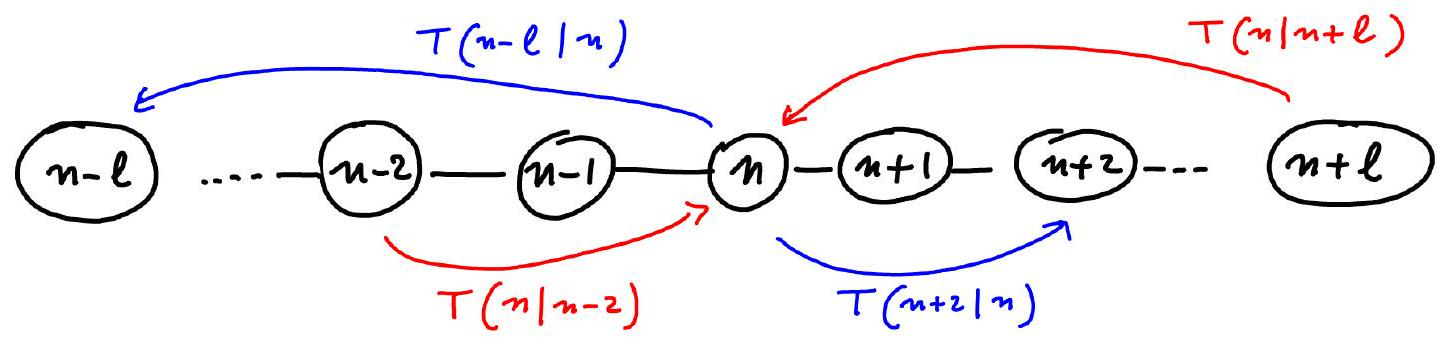
\includegraphics[width=0.5\textwidth]{2025_10_17_3daf2a002a8f5936c90eg-19}
\end{figure}
The M.E. for the propagator $p\left(n, t \mid n_{0}, t_{0}\right)$ is then
\begin{DispWithArrows}[displaystyle, format=c]
    P(n, t+\Delta t)=\underbrace{\sum_{m \neq n} T(n \mid m) \Delta t}_{\substack{\text { probability to } \\ \text { jump from any state } m \neq n \\ \text{ into the state } n}} P(m, t)+\underbrace{\left(1-\sum_{m \neq n} T(m \mid n) \Delta t\right)}_{\substack{\text{probability to} \\ \text{remain in the state } n}} P(n, t)
\end{DispWithArrows}
Therefore as $\Delta t \rightarrow 0$ the Master Equation becomes
\begin{DispWithArrows}[displaystyle, format=c]
    \frac{\partial}{\partial t} p(n, t)=\sum_{m}[T(n \mid m) p(m, t)-T(m \mid n) p(n, t)]
\end{DispWithArrows}
notice that we have included the state $n$ in the sum (why?).

As usual eq. (31) must be equipped with initial conditions $P\left(n, t_{0} \mid n_{0}, t_{0}\right)=\delta_{n, n_{0}}$ and, possibly, some boundary conditions.

Exercise: - Show that $\sum_{n} p(n, t)=1$.
\begin{itemize}
    \item Define the $l$-th jump moment as
    \begin{DispWithArrows}[displaystyle, format=c]
        \mu_{l}(n)=\sum_{m}(m-n)^{l} T(m \mid n) \quad l \geqslant 0
    \end{DispWithArrows}
    Show then that
    \begin{DispWithArrows}[displaystyle, format=c]
        \frac{d}{d t}\langle n\rangle=\left\langle\mu_{1}(n)\right\rangle \rightarrow \text { is this a closed eq. for }\langle n\rangle \text { ? }
    \end{DispWithArrows}
    \begin{DispWithArrows}[displaystyle, format=c]
        \frac{d}{d t}\left\langle n^{2}\right\rangle=\left\langle\mu_{2}(n)\right\rangle+2\left\langle n \mu_{1}(n)\right\rangle
    \end{DispWithArrows}
    where $\langle f(n)\rangle \equiv \sum_{n} f(n) p(n, t)$
\end{itemize}
As we have seen in eq. (4a) and (4b), we can define a matrix $\mathbb{W}$ whose entries are ($T(n \mid n)=0$)
\begin{DispWithArrows}[displaystyle, format=c]
    W_{n m}=T(n \mid m)-\sum_{l} T(l \mid n) \delta_{n, m}
\end{DispWithArrows}
which shows that $\mathbb{W}_{n m} \geq 0$ for $n \neq m$ and $\sum_{n} \mathbb{W}_{n m}=0$. The M.E. eq. (31) then reads
\begin{DispWithArrows}[displaystyle, format=c]
    \begin{gathered}
    \dot{\vec{p}}=W\vec{p} \quad \text { or } \quad \dot{p}_{n}=\sum_{m} \mathbb{W}_{n m} p_{m} \\
    \mathbb{W}=\left(\begin{array}{cccc}
     w_{11} & T(1 \mid 2) & T(1 \mid 3) & \ldots \\
     T(2 \mid 1) & w_{22} & T(2 \mid 3) & \ldots \\
     T(3 \mid 1) & T(3 \mid 2) & w_{33} & \\
     \vdots & \vdots & & \ddots
    \end{array}\right) \leftarrow \text { jumps from } m=2,3 \ldots \text { to } 1 \\
     w_{ii} \equiv-\sum_{m} T(m \mid i) \\
     \substack{\text { jumps from } \\
     1 \text { to } m=2,3, \ldots}
    \end{gathered}
\end{DispWithArrows}
We can find the stationary state by setting $\dot{P}_{n}=0$ From eq. (31):
\begin{DispWithArrows}[displaystyle, format=c]
    \sum_{m}\left[T(n \mid m) p_{st}(m)-T(m \mid n) p_{st}(n)\right]=0
\end{DispWithArrows}
This eq. is difficult to solve in general. However we can find the equilibrium solution if each and every term in the sum is zero (much stronger assumption). In this latter case we get
\begin{DispWithArrows}[displaystyle, format=c]
    T(n \mid m) P_{eq}(m)=T(m \mid n) P_{eq}(n) \quad \text{DETAILED BALANCE}
\end{DispWithArrows}
This assumption means that every state $m$ is balanced only by the state $n$, like in the birth
and death case, which in general is not true. All states are balanced in pairs. Of course, the detailed balance condition satisfies eq. (32), but eq. (32) does not imply eq. (33). In general one cannot impose eq. (33).

We again can connect this to stat. Mech. If
\begin{DispWithArrows}[displaystyle, format=c]
    P_{\text {eq. }}(n)=\frac{1}{z} e^{-\beta E(n)}
\end{DispWithArrows}
Where $E(n)$ is the energy of state $n$, then eq. (32) is satisfied if we choose $T(n \mid m)$ and $T(m \mid n)$ such that
\begin{DispWithArrows}[displaystyle, format=c]
    \frac{T(n \mid m)}{T(m \mid n)}=e^{-\beta(E(n)-E(m))}
\end{DispWithArrows}
Even though other choices are possible to satisfy detailed balance, eq. (33) allows us to describe a physical system at equilibrium with a heat bath at temperature $\beta^{-1}$.
